
\chapter{Bildkorrektur}

Ein bekanntes Problem der Computergrafik sind die Alias-Effekte. Zu den bekanntesten gehört die Treppenbildung an nahezu horizontal bzw. vertikal verlaufenden Kanten, oder der Moiré-Effekt bei dem z.B. durch Überlagerung zweier feiner Gitter ein gröberes Muster entsteht.
Beispiele hierfür liefert Abb. \ref{fig:midpoint}. So kann an den horizontal verlaufenden Linien des Schachbretts Treppenbildung beobachtet werde. Ebenso zeigt sich eine Form des Moiré-Effekt und zwar in den hinteren Reihen des Schachbretts, in denen Kacheln wieder größer werden.

Eine Erklärung für diese Erscheinungen findet man in der Signalverarbeitung. Dort tritt "`Aliasing"' auf, wenn das ursprüngliche Signal nicht mit einer ausreichend hohen Frequenz abgetastet wird, und deshalb nicht vollständig rekonstruiert werden kann. Um ein Signal fehlerfrei rekonstruieren zu können muss die Abtastfrequenz mindestens doppelt so hoch sein, wie die höchsten Frequenzanteile des Signals. Die Grenzfrequenz ab der eine fehlerfreie Rekonstruktion möglich ist, heißt Nyquist-Frequenz.

Im Kontext des "`Raytracing"' ist das Ursprungssignal eine kontinuierliche Funktion über,  auf den Sensor einfallender, Strahldichten. Dieses Signal wird an diskreten Punkten abgetastet. Bisher geschah dies, indem Strahlen durch den Mittelpunkt eines PEE geschossen wurden.
Zur Bildkorrektur schießt man durch ein einzelnes PEE mehrere Strahlen, um so die Abtastfrequenz zu erhöhen und das Ursprungssignal so gut wie möglich rekonstruieren zu können.

% Die Stellen an denen das PEE vom Strahl durchdrungen werden "`Samples"' genannt und das Verfahren zur Erzeugung der "`Samples"' als "`Sampling"' bezeichnet.


\section{Erzeugung geeigneter Abtastpunkte}

Das Verfahren zur Erzeugung weiterer Abtastpunkte auf den PEE wird auch als "`Sampling"' bezeichnet. Bevor die einzelnen "`Sampling"'-Verfahren vorgestellt werden, werden informell Sachverhalte aus der Signalverarbeitung erläutert, um besser nachvollziehen zu können, was beim "`Sampling"' beachtet werden sollte.

Multidimensionale Signale zeigen eine räumliche Änderung, wie z.B. die Verteilung der Strahldichten über die Projektionsebene. Solche Signale lassen sich als Funktionen im Ortsraum darstellen. Durch die Fourier-Transformation lassen sich Signale vom Ortsraum in den Frequenzraum transformieren. Hier wird sichtbar wie viele Anteile des Signals in einem bestimmten Frequenzband liegen. Das Signal dargestellt als Funktion wird abgetastet, indem die Funktion mit einem Dirac-Kamm multipliziert wird. Der Dirac-Kamm besteht aus einer Folge von Dirac-Stößen, die sich nach konstanten Perioden \( T \) der Abtastfrequenz wiederholen. Die Periode \( T \) hängt von der Anzahl der Abtastpunkten - den "`Samples"' - ab. Je mehr Abtastpunkte vorhanden sind desto kleiner ist \( T \). Dieser Prozess der Signalabtastung kann auch im Frequenzbereich beobachtet werden. Nur handelt es sich hier um eine Faltung des Frequenzspektrums mit einem Dirac-Kamm der Periode \( \frac{1}{T} \). Sind nicht genug Abtastpunkte vorhanden, überlagern sich Frequenzbereiche des Signals. Diese Überlagerungen im Frequenzraum lassen sich nicht mehr fehlerfrei rekonstruieren.

Zwei Dinge versucht man deshalb bei den "`Sampling"'-Verfahren zu erreichen.
Einerseits kann das Überlappen von Frequenzbereichen im Frequenzraum reduziert werden, indem man mehr Strahlen durch ein PEE schießt und so die Anzahl an Abtastpunkten erhöht, denn dies vergrößert die Abstände der Dirac-Stöße im Frequenzraum. Dennoch ist es möglich, dass sich Überlappungen nicht komplett verhindern lassen, weil dazu zu viele "`Samples"' benötigt werden, was sich linear in der Laufzeit niederschlägt. In diesem Fall versucht man die Regelmäßigkeit, mit der Abtastpunkt auf Abtastpunkt folgt, zu stören. Denn diese Regelmäßigkeit verursacht die störenden Alias-Effekte und Bildartefakte. Ziel ist es daher das PEE möglichst mit geringer Diskrepanz (das heißt die "`Samples"' sollten einen möglichst großen Abstand zueinander haben) jedoch nicht regelmäßig durch "`Samples"' aufzuteilen. Dadurch werden Alias-Effekte und Bildartefakte durch Rauschen ersetzt, was für den Betrachter natürlicher wirkt.

\begin{itemize}
    \item Mittelpunkt "`Sampling"': Die einfachste Art des "`Sampling"', indem durch den Mittelpunkt eines PEE ein Primärstrahl geschossen wird. Abb.~\ref{fig:midpoint} zeigt durch die geringe und regelmäßige Abtastung Treppenbildung an Kanten und Schatten des Buddhas, sowie horizontal und vertikal verlaufenden Kanten der Kacheln. Nahe des Horizonts kommt es zu Bildartefakte durch wieder größer werdende Kacheln.
    
    \item "`Random Sampling"': Die Komponenten eines "`Samples"' werden gleichverteilt entlang der x-und y-Achse des PEE gezogen. Abb.~\ref{fig:random4} zeigt den Ausschnitt mit 4 "`Samples"'. Durch das komplett zufällige ziehen der "`Samples"', kann es zu schlechten Verteilungen durch Pulk Bildung kommen. Zwar wurde die Treppenbildung entfernt, dafür erscheinen Kanten und Schatten ausgefranst. Die hinteren Bildartefakte wurden durch Rauschen ersetzt.
    
    \item "`Stratified Sampling"': Das PEE wird in kleinere gleichgroße Quadrate unterteilt. Innerhalb dieser Quadrate wird je ein "`Sample"' durch "`Random Sampling"' erzeugt. Abb.~\ref{fig:stratified4} zeig den Ausschnitt mit 4 "`Samples"'. Der Ausschnitt ähnelt sehr dem des "`Random Sampling"', jedoch mit weniger Rauschen, da durch die weitere Aufteilung des PEE die Pulk-Bildung verhindert wird.
    
    \item "`Hammersley Sampling"': Aus \( n \) zu erzeugenden "`Samples"' berechnet sich die erste Komponente des \( i \)-ten "`Samples"' aus \( \frac{i}{n} \) und die zweite aus dem \( i \)-ten Element der "`Van der Corput"' Zahlenreihe zur Basis 2. Abb.~\ref{fig:hammersley4} zeigt bei 4 "`Samples"' bessere Glättung der Kanten als "`Random"' oder "`Stratified"' Sampling, da kein ausfransen zu erkennen ist. Es zeichnet sich durch geringe Diskrepanz und unregelmäßiger Verteilung der "`Samples"' aus. Jedoch fehlt der Zufallsfaktor bei diesem Verfahren, was neue Alias-Effekte anstelle von Rauschen ins Bild einbringt. Dies wird durch 2 graue Streifen in der Nähe des Horizonts deutlich.
    
   
\end{itemize}


\newpage

\begin{center}
\begin{minipage}[t]{0.72\textwidth}
    \centering
    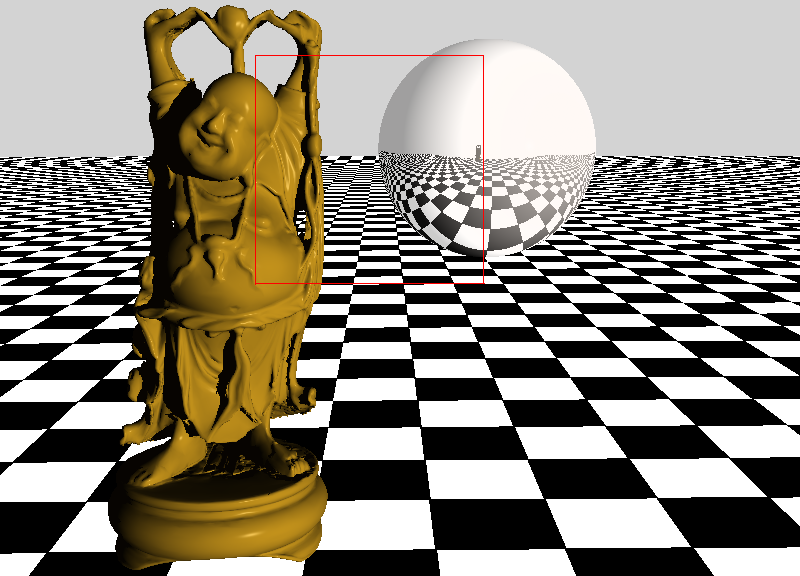
\includegraphics[width=\textwidth]{./img/bildkorrektur/midpoint_ganz.png}
    \captionof{figure}{Komplette Szene "`gerendert"' mit Mittelpunkt "`Sampling"'. Die folgenden Ausschnitte verwenden unterschiedliche "`Sampling"' Verfahren. Die Zahl steht für die Anzahl verwendeter "`Samples"'.}
    \label{fig:midpoint_ganz}
\end{minipage}
\end{center}
\begin{minipage}[t]{0.33\textwidth}
    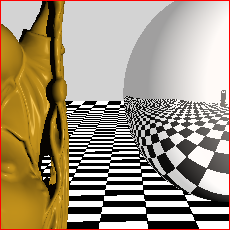
\includegraphics[width=\textwidth]{./img/bildkorrektur/midpoint.png}
    \captionof{figure}{1 Mittelpunkt}
    \label{fig:midpoint}
\end{minipage}
\begin{minipage}[t]{0.33\textwidth}
    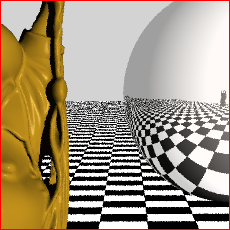
\includegraphics[width=\textwidth]{./img/bildkorrektur/random4.png}
    \captionof{figure}{4 "'Random"'}
    \label{fig:random4}
\end{minipage}
\begin{minipage}[t]{0.33\textwidth}
    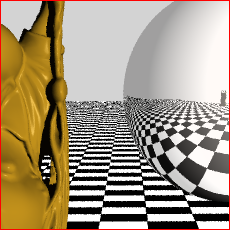
\includegraphics[width=\textwidth]{./img/bildkorrektur/stratified4.png}
    \captionof{figure}{4 "'Stratified"'}
    \label{fig:stratified4}
\end{minipage}\\
\begin{minipage}[t]{0.33\textwidth}
    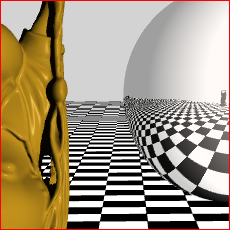
\includegraphics[width=\textwidth]{./img/bildkorrektur/hammersley4.png}
    \captionof{figure}{4 "'Hammersley"'}
    \label{fig:hammersley4}
\end{minipage}
\begin{minipage}[t]{0.33\textwidth}
    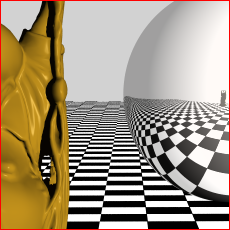
\includegraphics[width=\textwidth]{./img/bildkorrektur/stratified64.png}
    \captionof{figure}{64 "`Stratified"'}
    \label{fig:stratified64}
\end{minipage}
\begin{minipage}[t]{0.33\textwidth}
    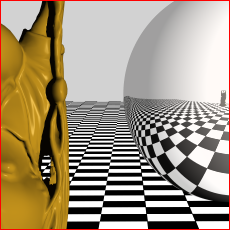
\includegraphics[width=\textwidth]{./img/bildkorrektur/hammersley64.png}
    \captionof{figure}{64 "`Hammersley"'}
    \label{fig:hammersley64}
\end{minipage}

\FloatBarrier
